\chapter{サービス設計}

\section{サービス概要}
前節で述べたビジネスモデルをもとに2013年9月下旬からwordpressを活用し、サービスの開発を開始した。開発と並行し、株式会社手嶋屋に協賛企業としてプロジェクトに参加して頂き、彼らのサービスであるオリジナルのソーシャルネットワークを作成できるpne.jpとクレジットカードを使ってクラブ活動の毎月の集金を自動化することができるpne.clubをプロジェクトに無性に提供して頂いた。

【協賛企業】

企業名:株式会社手嶋屋
サイト:http://www.tejimaya.com/
協賛内容:ソーシャルネットワーク作成ツールpne.jpとクラブ集金ツールpne.clubの無償提供
\section{サービスコンセプト}
サービスのローンチにあたり、Liven Upのサービスコンセプトを「手軽に格安でフットサルの試合を組めるプラットフォーム」とした。本サービスで試合をマッチングすることで、フットサルコートのアイドリングタイムを手間をかけずに有効に活用できることを目標とした。

\begin{itemize}
	\item フットサルプレイヤーは、簡単にフットサルの試合相手を見つけることができ、格安で参加できる。
	\item コートは効率的に空きコートを埋めることができる
	\item 参加者のみで試合を運営できる
\end{itemize}
\section{サイトデザイン}
\subsection{トップページ}
トップページでは図で示した通り、一目で各フットサルコートの情報を訴えかけられるように各フットサルコートを並べて、利用者の立地条件が一番コートを選んでもらえるようにした。予約のタブを押すと利用者が予約したい日時を決めるページに飛ぶ。
\\
\\
\\
\\
\\
\begin{figure}[htbp]
	\centering
	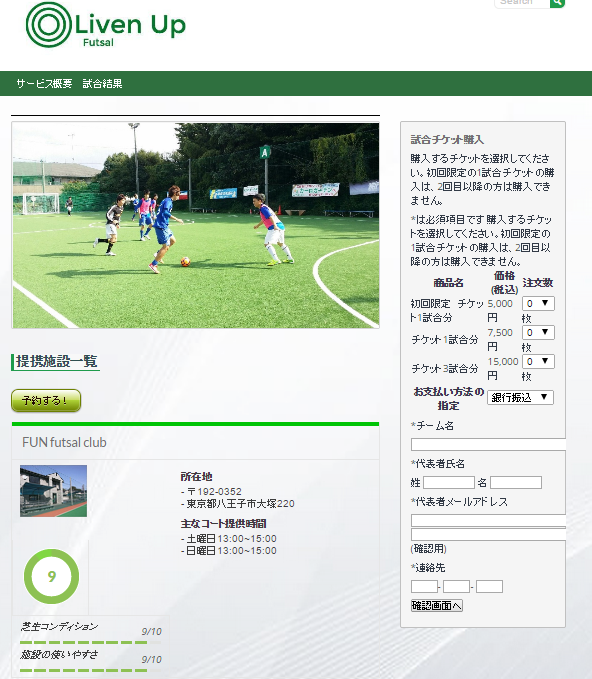
\includegraphics[width=85mm, bb=10 0 500 300]{figures/top.jpg}
	\caption{施設情報 {\itshape Google Map}}
	\label{施設情報}
\end{figure}

\newpage

\subsection{チケット購入ページ}
画面右には本サイト内で購入できるチケットの購入ページを配置した。初回のみ5000円で購入できるが、2回目以降は一回7500円、3試合分のチケットをまとめて購入すると15000円で購入できる。まとめて購入してもらうことにより多くのチームに試合に参加できる選択肢を持たせる価格設定にした。
\\
\\
\\
\\
\\
\\
\begin{figure}[htbp]
	\centering
	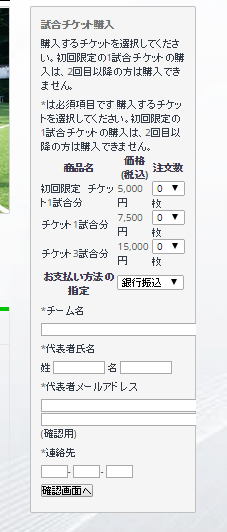
\includegraphics[width=85mm, bb=30 0 300 300]{figures/buy.jpg}
	\caption{購入画面 {\itshape Google Map}}
	\label{購入画面}
\end{figure}
\newpage


\subsection{フットサルコート情報}
フットサルコートの情報を所在地やコートの主な使用できる時間帯、各指標を示した。また気に入ったらワンタッチで予約ができるように予約タブを配置した。
\ 次のページで、予約可能の日時一覧が出てきて、新たに予約できる都合の良い日時にエントリーできるようになっている。
\\
\\
\\
\\
\\
\begin{figure}[htbp]
	\centering
	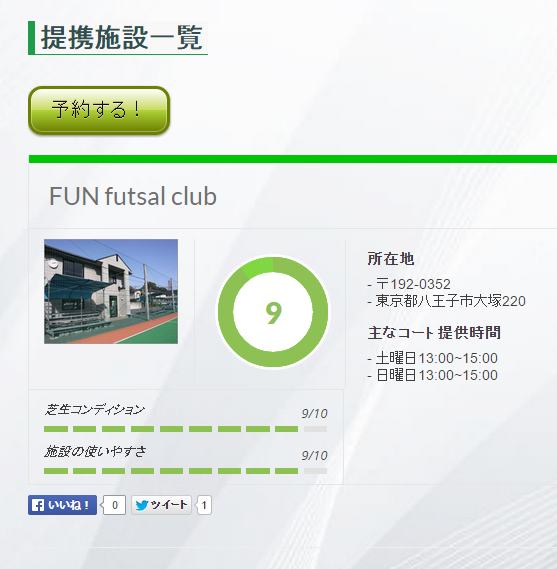
\includegraphics[width=85mm, bb=0 0 300 300]{figures/book.jpg}
	\caption{施設情報 {\itshape Google Map}}
	\label{施設情報}
\end{figure}
\newpage
\begin{figure}[htbp]
	\centering
	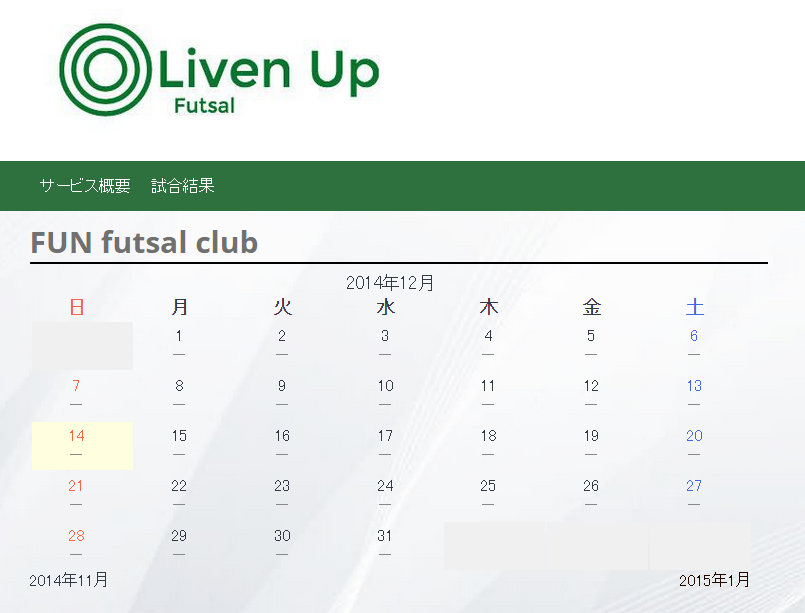
\includegraphics[width=85mm, bb=0 0 400 300]{figures/date.jpg}
	\caption{予約画面 {\itshape Google Map}}
	\label{予約画面}
\end{figure}
\newpage



\section{ステークホルダー別サービス利用フロー}
本節では本サービスのステークホルダーのサービス利用フローについて説明する。

\subsection{フットサルコートの利用フロー}
フットサルコートのオーナーは1章のインタビューでもあった通り、できるだけにクーポン出稿に際した文言や手間を省いた。
\\ 先にも紹介した通り、各フットサルコートのページは固定であり、フットサルコートのオーナーは主に本サイトのメールアドレスにコートが予約が入っていない時間帯を送るだけである。
\\ 本サイトのスタッフでフットサルコートの予約できる時間帯を随時更新していき、予約が埋まり次第、コートに電話をし、コート抑え、翌日営業以内に送金をする仕組みである。


\subsection{プレイヤーの利用フロー}
 購入ページからチケットを購入したのちに、各コートの予約ページから都合のよい時間帯を選び予約する。
 \\ 予約をしてから3日ごとに利用者に報告するようしている。成立する場合でも4日前までには連絡する仕組みである。